\documentclass[12pt]{beamer}
\usepackage{amssymb,amsmath,amsthm}
\usepackage[utf8x]{inputenc}
\usepackage{graphicx}
\usepackage{siunitx}
\usepackage{tikz}
\setcounter{secnumdepth}{0}
\usetheme{Berkeley}
\usecolortheme{seagull}
\usepackage{xcolor}
\def\myEmail{hxr@hx42.org}
\def\InternalGithub{erasche}

\def\myGithub{@\InternalGithub}
\def\myGithubUrl{https://github.com/\InternalGithub}
\def\myName{Helena Rasche}


\title[Phage Annotation]{Interactive Annotation of Bacteriophage Genomes}
\author[\myName]{\myName\ \\\ \\Center for Phage Technology\ \\Texas A\&M University}
\date{2016-03-18\ \\
\includegraphics[width=31pt]{cc-by-sa.png}}
\usepackage{hyperref}
\usepackage{cleveref}

\begin{document}
\frame{\titlepage}

\section{Who}
\begin{frame}{Who Am I / CPT}
    \begin{itemize}
    \item Systems Administrator, Programmer, Bioinformatician
    \item Worked at the CPT for $\approx$3 years
    \item Completely rewrote org's practices on genome annotation
    \item $\approx$160 tools/wrappers developed
        \begin{itemize}
            \item 94 Phage specific
            \item 28 for external services (NCBI, Apollo)
            \item 26 Other (Small utilities, NGS, comparative genomics, scripts)
        \end{itemize}
    \item Working on next generation of genome annotation infrastructure
    \end{itemize}
\end{frame}

\begin{frame}{Who Am I / Galaxy}
    \begin{itemize}
        \item Co-developer of Galaxy Interactive Environments
        \item Galaxy Committer
            \begin{itemize}
                \item Involved in: cargo-port, starforge, planemo, pulsar, galaxy
            \end{itemize}
        \item Galaxy Tool Developer
        \begin{itemize}
            \item JBrowse in Galaxy
            \item NCBI Entrez Suite
            \item HMMER3 Suite
            \item ART
            \item Seqtk suite
            \item progressiveMauve
        \end{itemize}
    \end{itemize}
\end{frame}

\begin{frame}{JBrowse}
    \centering
    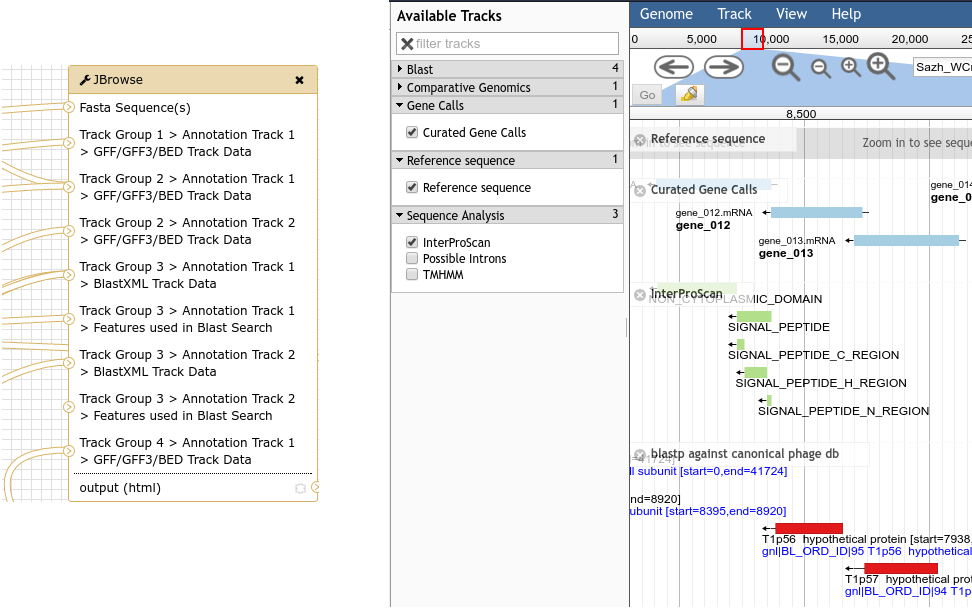
\includegraphics[width=\textwidth]{./jigc.png}
\end{frame}


\section{Phages}
\begin{frame}{Bacteriophages / Background}
    \begin{itemize}
        \item Viruses which attack bacteria
        \item Some are lytic, some are lysogenic
    \end{itemize}
    \centering
    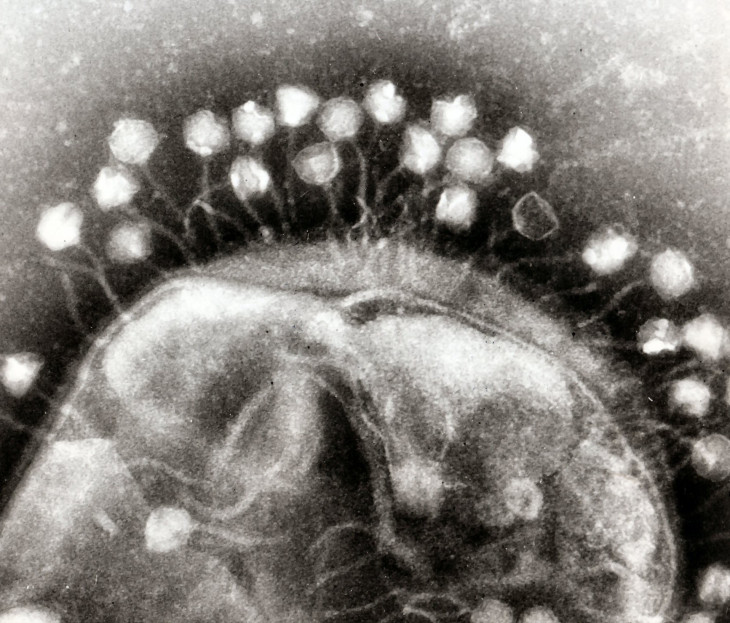
\includegraphics[]{./phage-attack.jpg}
\end{frame}
\begin{frame}{Caudovirales}
    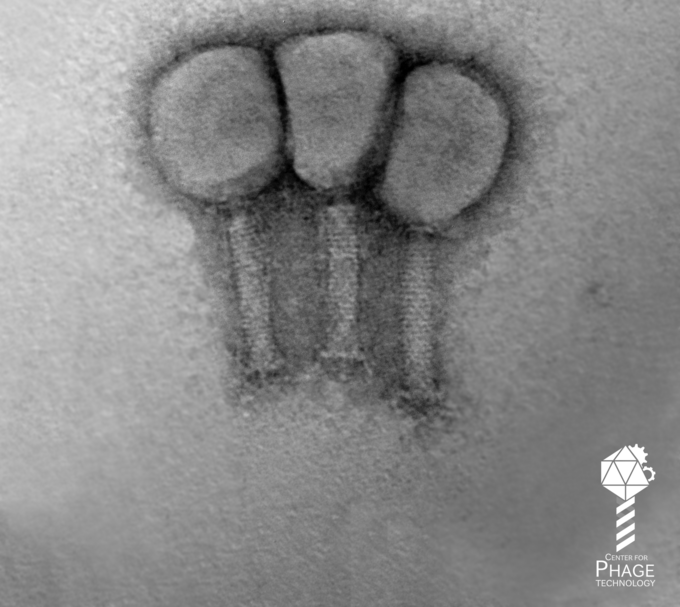
\includegraphics[height=\textheight]{./triplets.png}
    %\item Caudovirales--most important type
    %\item Linear, dsDNA genomes
    %\item \SIrange{16}{>600}{kb}
\end{frame}
\begin{frame}{Myoviridae, Podoviridae, and Siphoviridae}
    \centering
    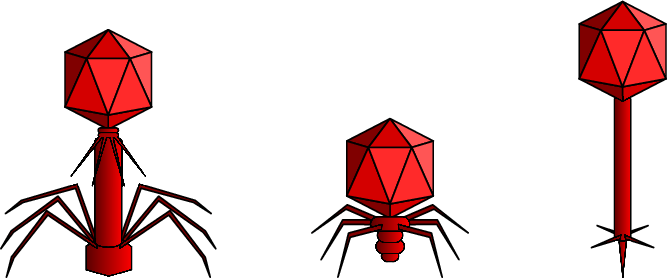
\includegraphics[width=\textwidth]{./Caudovirales.png}
    %\cite[File:Caudovirales]
\end{frame}

\begin{frame}{Why they're great}
    \begin{itemize}
        \item Very practical organism to study
        \item Grow quickly (200 virions per 20 minutes)
        \item Small, easy to annotate
    \end{itemize}
    \centering
    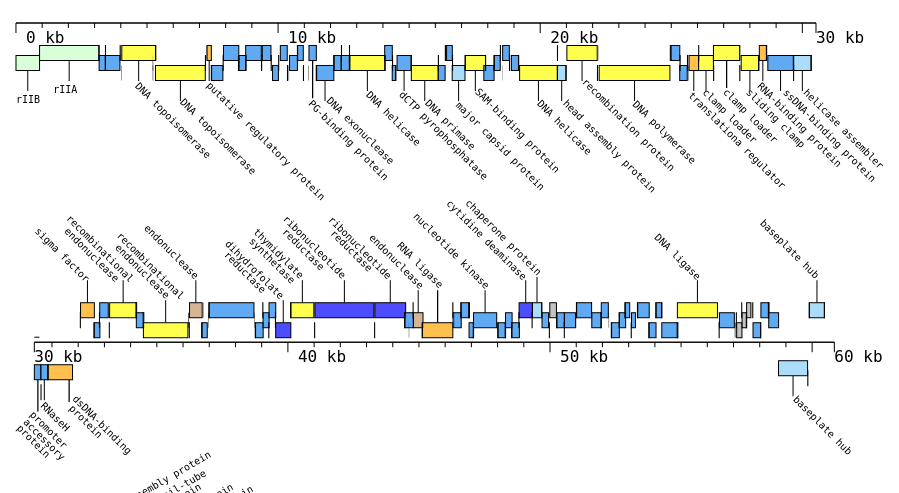
\includegraphics[height=.5\textheight]{./annotation.png}
\end{frame}

\section{Who Cares}
\begin{frame}{Coming Wave of Phage Genomics}
    \begin{itemize}
        \item Phages are incredibly diverse
        \item Relatively poor representation in databases
        \item Very practical organism
        \item Phage Therapy \& end of antibiotic era
    \end{itemize}
\end{frame}
\begin{frame}{Phage Therapy}
    \begin{itemize}
        \item Cannot contain generalized transducers
        \item Cannot be lysogenic
        \item Cannot contain toxin genes
        \item $\implies$ need well annotated phages
    \end{itemize}
    \centering
    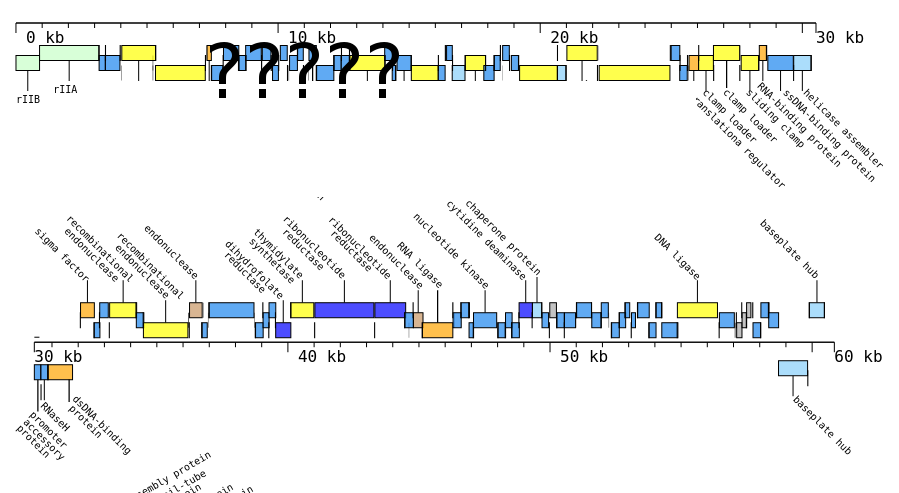
\includegraphics[height=.5\textheight]{./therapy.png}
\end{frame}

\section{Annotation}
\begin{frame}{Special Problems of Phage Genomics}
    \begin{itemize}
        \item High gene density, lots of overlap
        \item Small genomes, cost effective sequencing?
    \end{itemize}
    \centering
    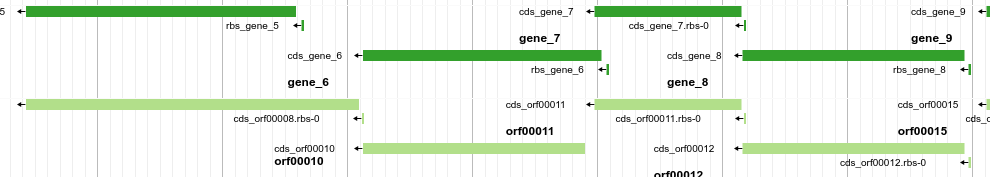
\includegraphics[width=\textwidth]{./overlap.png}
\end{frame}

\begin{frame}{Special Problems of Phage Genomics}
    \begin{itemize}
        \item Mosaic structure issues
        \item High mutation rates, 10-100X bacteria
        \item High diversity + high recombination $\implies$ nearly total lack of reference genomes
    \end{itemize}
    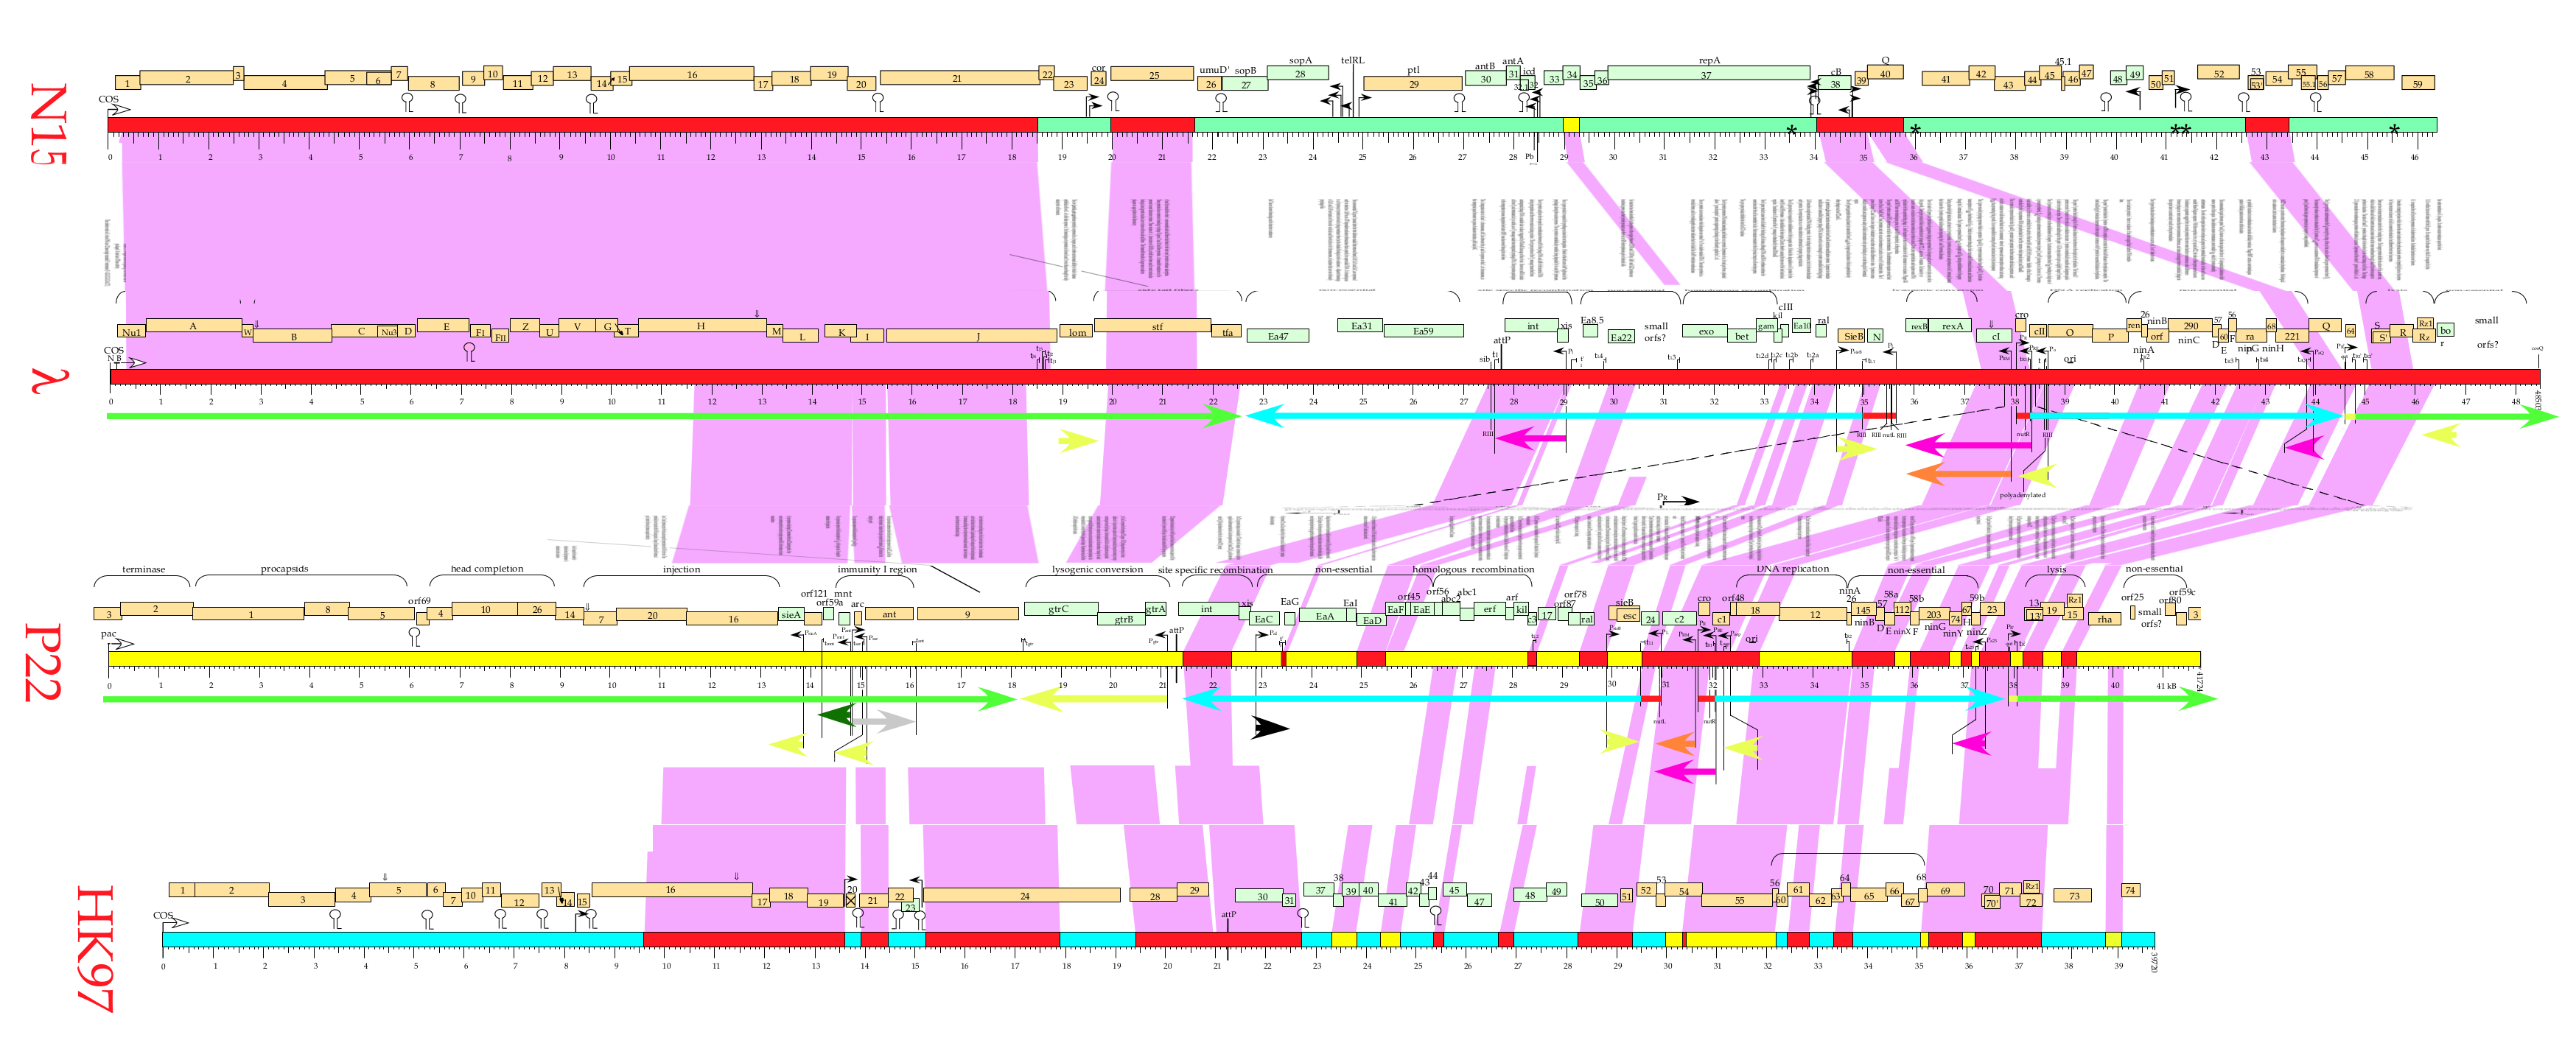
\includegraphics[width=\textwidth]{./ALOID.png}
\end{frame}

\begin{frame}{Special Problems of Phage Genomics}
    \begin{itemize}
        \item Modify RNApol or encode own, identifying promoters impossible
        \item Morons inserted in transcripts with independent promoters/terminators
    \end{itemize}
    \centering
    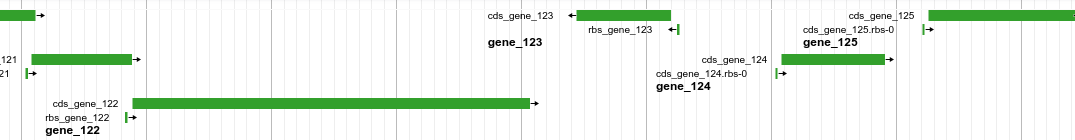
\includegraphics[width=\textwidth]{./morons.png}
\end{frame}

\begin{frame}{More Problems: Prophages}
    \begin{itemize}
        \item Vast majority of ``phage'' gene sequencse in prophages
        \item $\approx$6 prophage elements per bacterial genome
        \item Skewed BlastP results
        \item Functionality of prophage genes unknown
    \end{itemize}
\end{frame}

\begin{frame}{More Problems: Historical}
    \begin{itemize}
        \item Inch wide, mile deep
        \begin{itemize}
            \item Almost all actual experiments done on few paradigms
            \item Everything else ``known'' via computation methods
        \end{itemize}
    \end{itemize}
\end{frame}

\begin{frame}{More Problems: Historical}
    \begin{itemize}
        \item Within that inch\ldots
        \begin{itemize}
            \item Each paradigm phage had own community
            \item Each community had own (conflicting) terminology
        \end{itemize}
    \end{itemize}
    \centering
    
\includegraphics[width=0.6\textwidth]{./standards.png}
\end{frame}

\begin{frame}{More Problems: Competing Groups}
    \begin{table}
        \begin{tabular}{lll}
            Term         & Phage & Meaning\\\hline
            \textbf{LTF} & T4    & Long Tail Fiber\\
                         & T5    & L-shaped Tail Fiber\\
            \textbf{STF} & T4    & Short Tail Fiber \\
                         & T5    & Side Tail Fiber\\
        \end{tabular}
    \end{table}
\end{frame}

\begin{frame}{More Problems: Automation}
    \begin{itemize}
        \item Historical gene naming issues
        \item Renaming fiasco (lambda, T7), cross referencing papers is tough
        \item Mutation rate
        \item Little to no ontology based annotation
    \end{itemize}
\end{frame}

\begin{frame}{Redeeming Qualities for Annotation?}
    \begin{itemize}
        \item Every caudovirales has list of mandated genes (MCP, portal, scaffolding protein, holin, endolysin, spanin)
        \item Proteins usually clustered (to avoid segregation by high rec rate)
        \item Genomic position/neighbours are important and preserved
        \item High rec rate forces domains close to each other
        \item Mosaicism can help infer functionality of regions
    \end{itemize}
\end{frame}

\section{Solutions}
\begin{frame}{Undergraduates!}
    \begin{itemize}
        \item We train them as phage annotators, they annotate a phage genome in a semester
        \item Human brain power until AI/software develops further
    \end{itemize}
    \centering
    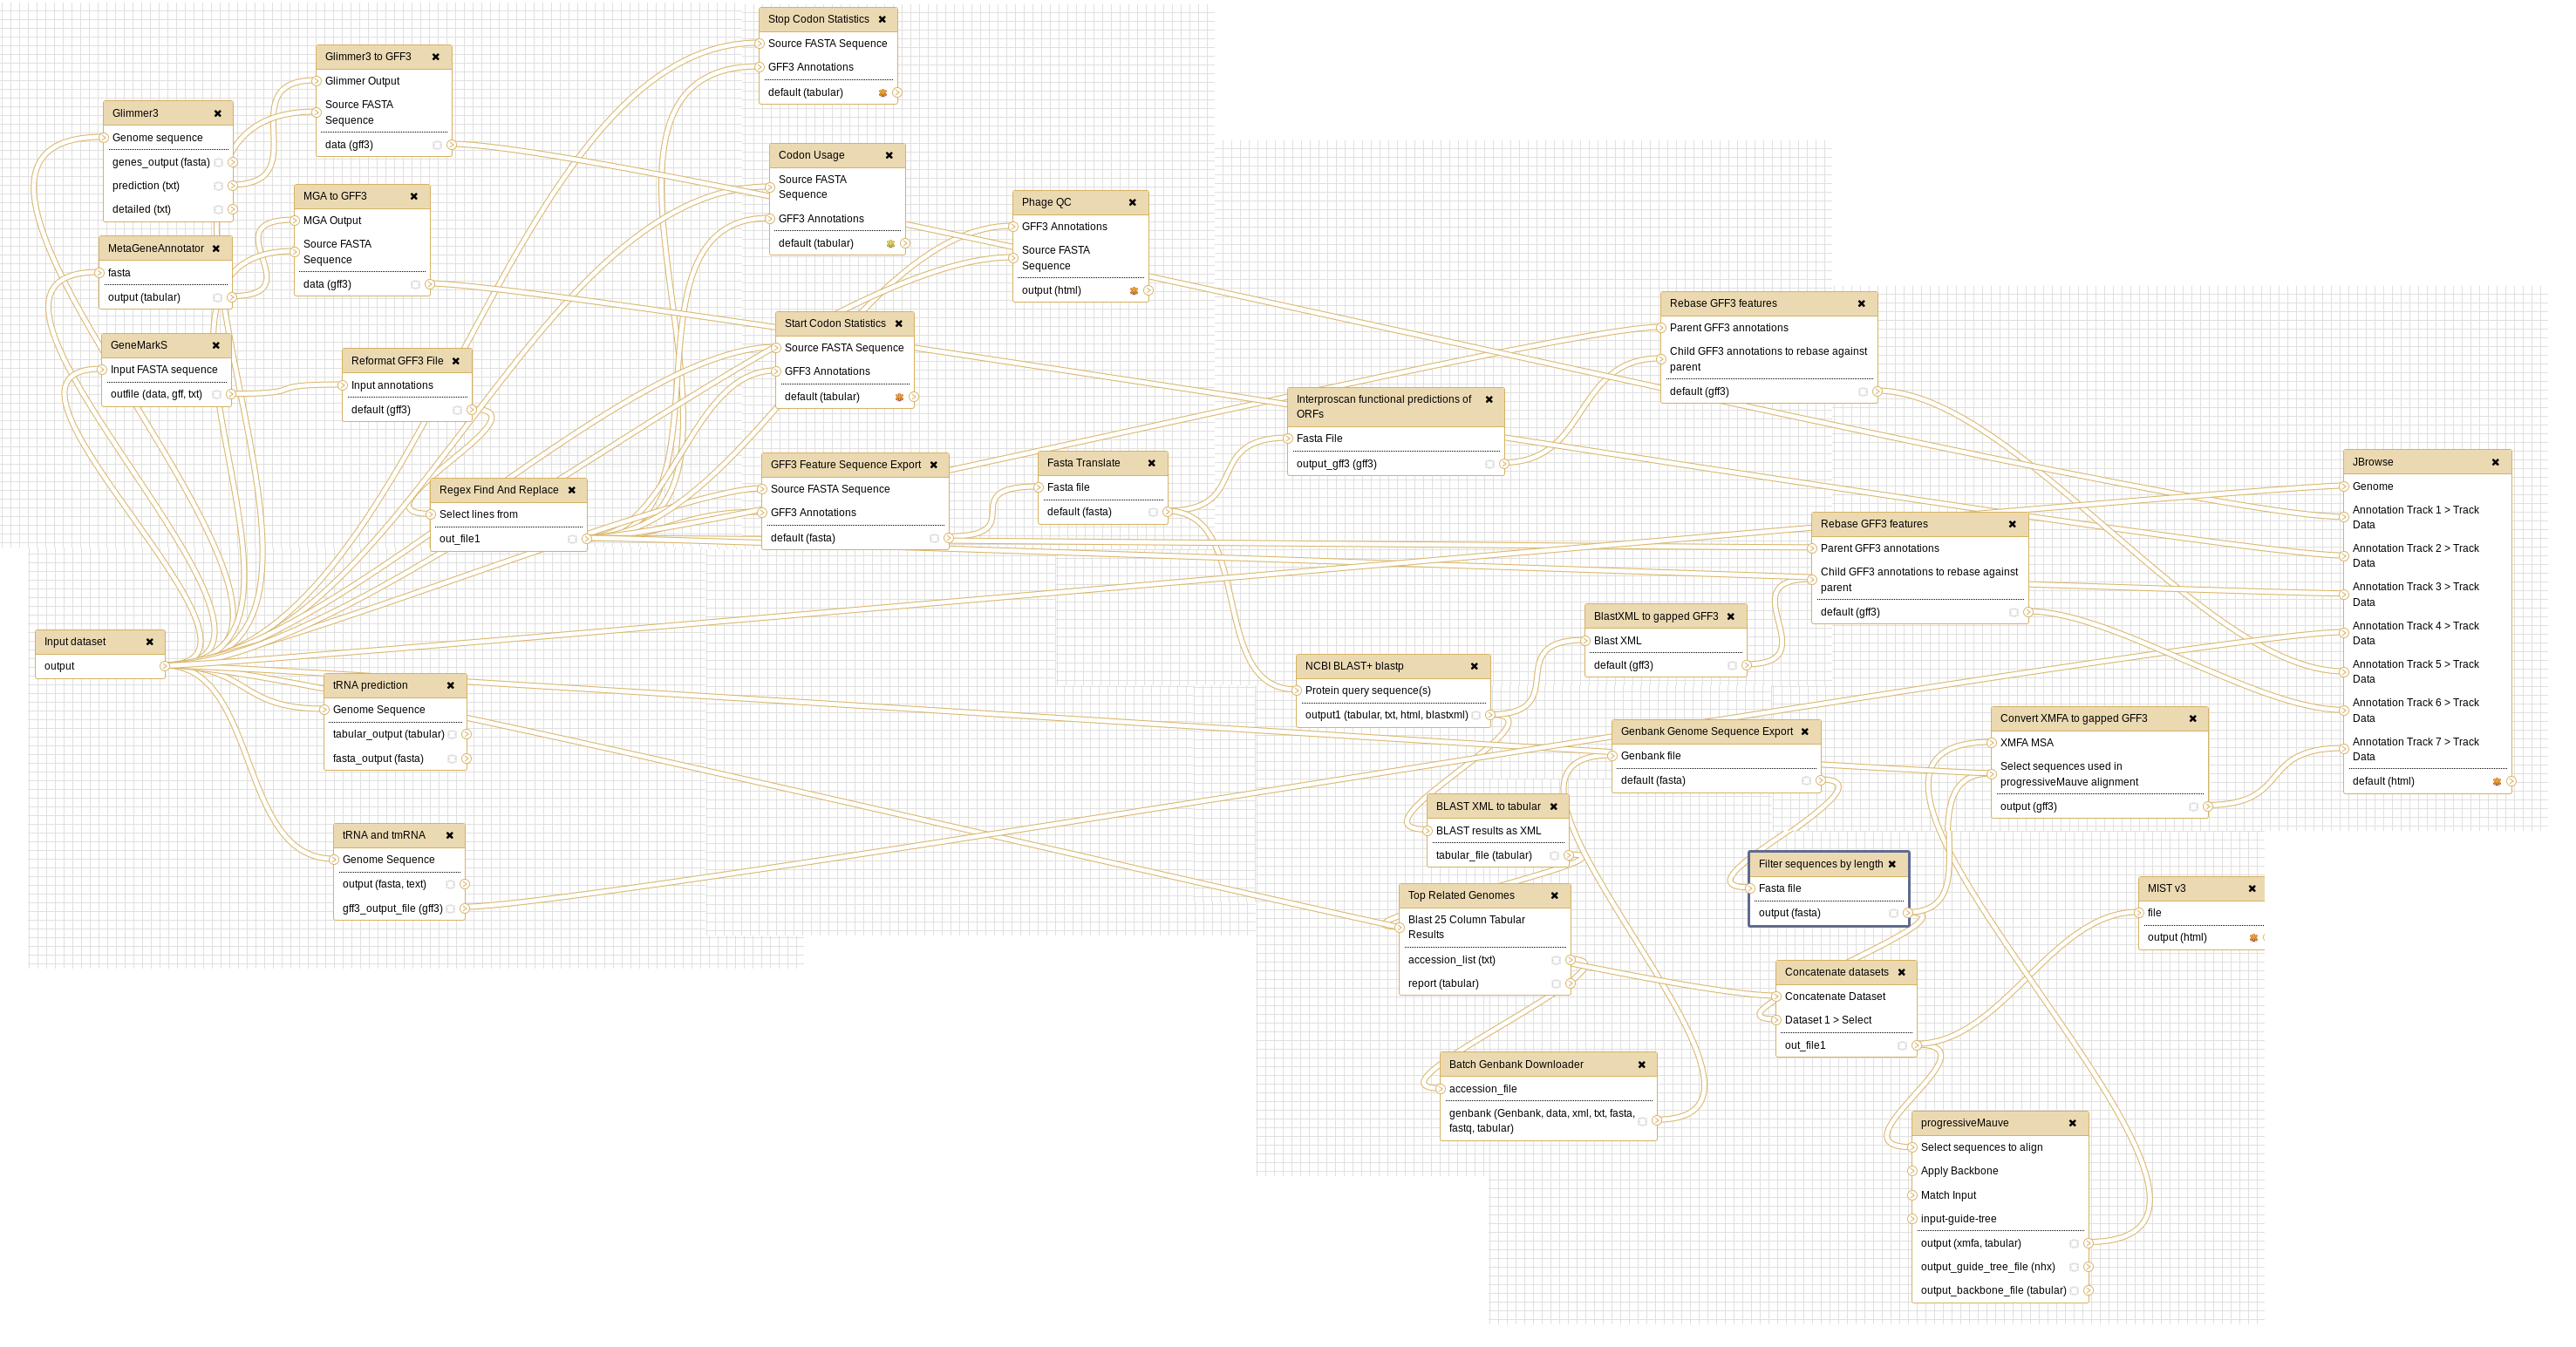
\includegraphics[width=\textwidth]{./pap2016.png}
\end{frame}

\begin{frame}{Automation}
    \begin{itemize}
        \item Great test bed for automation
        \item Software is \emph{not} time/memory/CPU constrained
        \item GO can be incredibly useful
    \end{itemize}
\end{frame}


\section{Annotation}


\begin{frame}{Apollo}
    \begin{itemize}
        \item Genome Annotation Client
        \item ``Google Docs'' of Genome annotation
        \item Only way forward for annotation efforts. Everyone should use it.
    \end{itemize}
\end{frame}

\begin{frame}{Apollo}
    \centering
    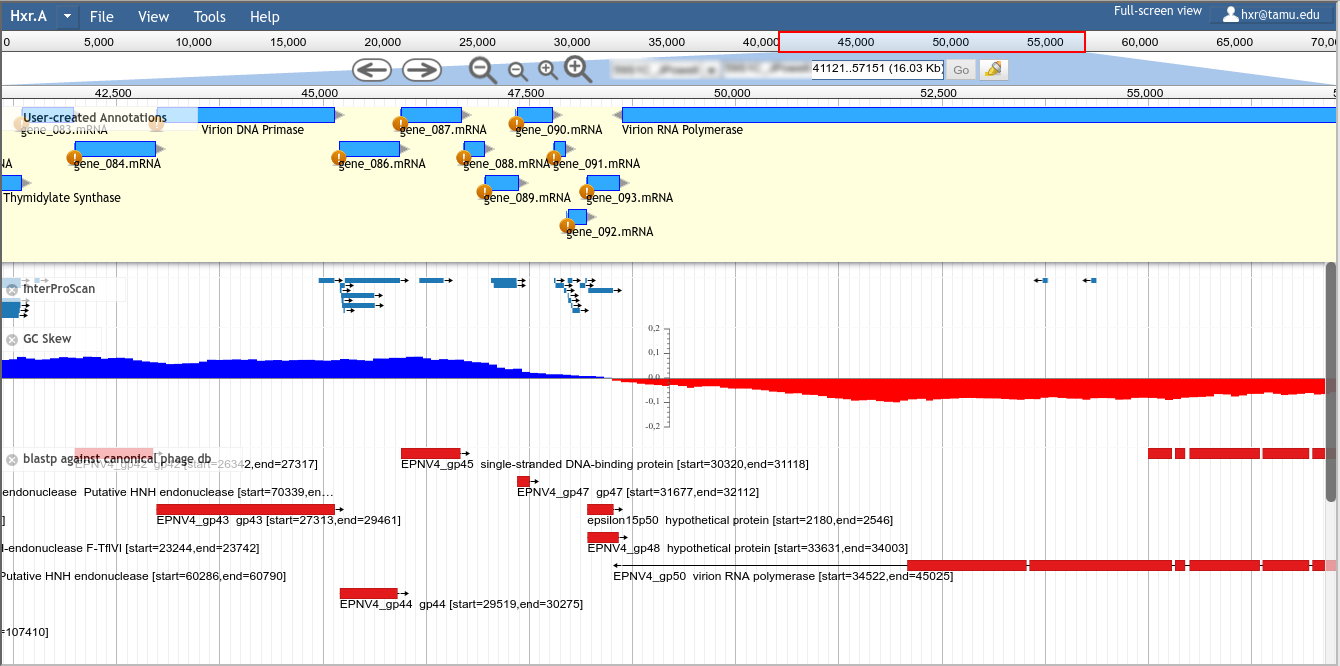
\includegraphics[width=\textwidth]{./apollo.png}
\end{frame}

\begin{frame}{Annotation in Practice}
    \begin{theorem}
        \begin{equation}
            \text{Galaxy} + \text{Apollo} = \text{\texttt{<3}}
        \end{equation}
    \end{theorem}
    \begin{proof}
        \begin{enumerate}
            \item Have shaved 5 weeks off of course
            \item Replaced with deeper dives into software
            \item Added new activities
        \end{enumerate}
    \end{proof}
\end{frame}

\begin{frame}{Annotation in the Future}
    \begin{theorem}
        \begin{equation}
            \text{Galaxy} + \text{Apollo} = \text{\texttt{<3}}\cdot10^{10^{10}}
        \end{equation}
    \end{theorem}
    via Galaxy Credentials for Remote Services
\end{frame}

\begin{frame}{Annotation in our Course}
    Two main parts:
    \begin{itemize}
        \item Structural annotation
        \item Functional annotation
    \end{itemize}
\end{frame}

\begin{frame}{Data Movement}
    \begin{figure}[!hb]
        \centering
        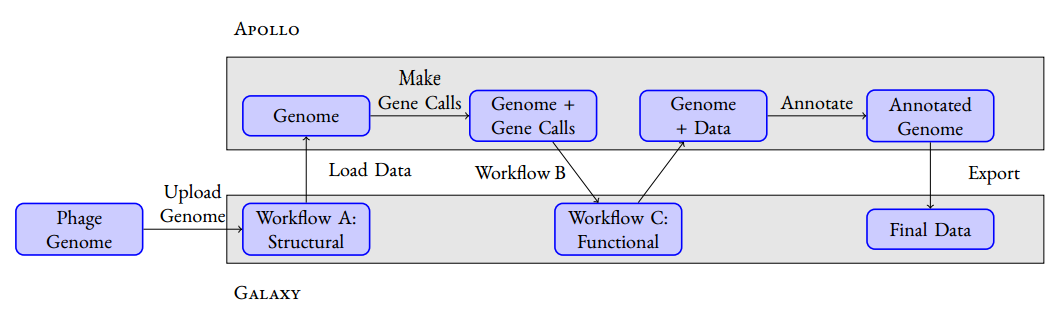
\includegraphics[width=\textwidth]{./ga.png}
        \caption{The data pathway through Apollo, Galaxy, and time}
    \end{figure}
\end{frame}


\section{Demo}
\begin{frame}{Demo}
    \begin{itemize}
        \item Quick demo of Apollo's functionality
    \end{itemize}
\end{frame}


\section{Q\&A}
\begin{frame}{Q\&A}
    \begin{itemize}
        \item Thank you for your time!
        \item Questions?
    \end{itemize}
\end{frame}

\end{document}
